% template taken from https://www.dickimaw-books.com/latex/admin/html/leafletcls.shtml

\documentclass[a4paper,12pt,notumble]{leaflet}

\usepackage[utf8]{inputenc}
\usepackage[T1]{fontenc}
\usepackage{tgadventor}

\usepackage{wasysym}
\usepackage{xcolor}
\usepackage{graphicx}
\usepackage{tikz}
\usepackage[utf8]{inputenc} 

\usetikzlibrary{calc}
\usetikzlibrary{shapes}
\usetikzlibrary{positioning,arrows}

\renewcommand*{\sectfont}{\scshape}
\renewcommand*{\descfont}{\bfseries\scshape}

\definecolor{rwth-blue}{HTML}{00549F}
\definecolor{rwth-lblue}{HTML}{8EBAE5}
\definecolor{rwth-llblue}{HTML}{C7DDF2}

\AddToBackground{1}{%
	\put (0,0) {
		
\begin{tikzpicture}
			\shadedraw[inner color=white,outer color=gray!20!white,draw=rwth-blue] (0,0) rectangle ($(\paperwidth, \paperheight)-(4pt,0pt)$);
		\end{tikzpicture}
	}
}

\AddToBackground{3}{%  Background of a small page
	\put(0,0){
		
\begin{tikzpicture}
			\draw[fill=rwth-llblue] (0,0) rectangle ($(2*\paperwidth, \paperheight)-(4pt,0pt)$);
		\end{tikzpicture}
	}
}

%%% Document start -------------------------------------------------------------------------
\begin{document}

%%%%%%%%%%%%%%%%%%
%%% Title page %%%
%%%%%%%%%%%%%%%%%%
\begin{center}


\includegraphics[height=1.25cm]{../Logos/Cosima18.png}

\vfill

% Schriftzug

\includegraphics[scale=0.25]{../Logos/GestikulaserSchriftzugOhneHut.png}

\vfill

\normalsize

\begin{tabular}{c}
	%Ein Projekt im Rahmen des \\
	%COSIMA-Wettbewerbs 2018
	Die neue Möglichkeit \\
	der Gestenerkennung
\end{tabular}

\vfill

\includegraphics[scale=0.25]{../Logos/GestikulaserLogoBuntOhneSchrift.png}
\vfill

\begin{tabular}{c}
	entwickelt von \\ \\
	Christoph Behr \\
	Cailing Fu \\
	Nicole Grubert \\
	Anna Pryadun \\
	Daniel Wolff
\end{tabular}

\vfill


\includegraphics[height=1.25cm]{../Logos/TOS.eps}

\end{center}

\newpage
\raggedright


%%%%%%%%%%%%%%%%%%%
%%% Second page %%%
%%%%%%%%%%%%%%%%%%%

\noindent
\begin{minipage}[c][0.58\textheight][t]{\textwidth}

	\section{Der Gestikulaser}

	Der Gestikulaser stellt eine neue Art der Gestenerkennung dar. Dabei wird die Hand des Nutzers, während er eine Geste macht, von Infrarot-LEDs beleuchtet und 
	das reflektierte IR-Licht mit Hilfe von Photodioden detektiert. Das entstandene Reflektionsmuster wird dann von einem neuronalen Netzmodell ausgewertet und 
	einer Geste zugeordnet. 
	
	\vspace{0.5cm}

	\centering
	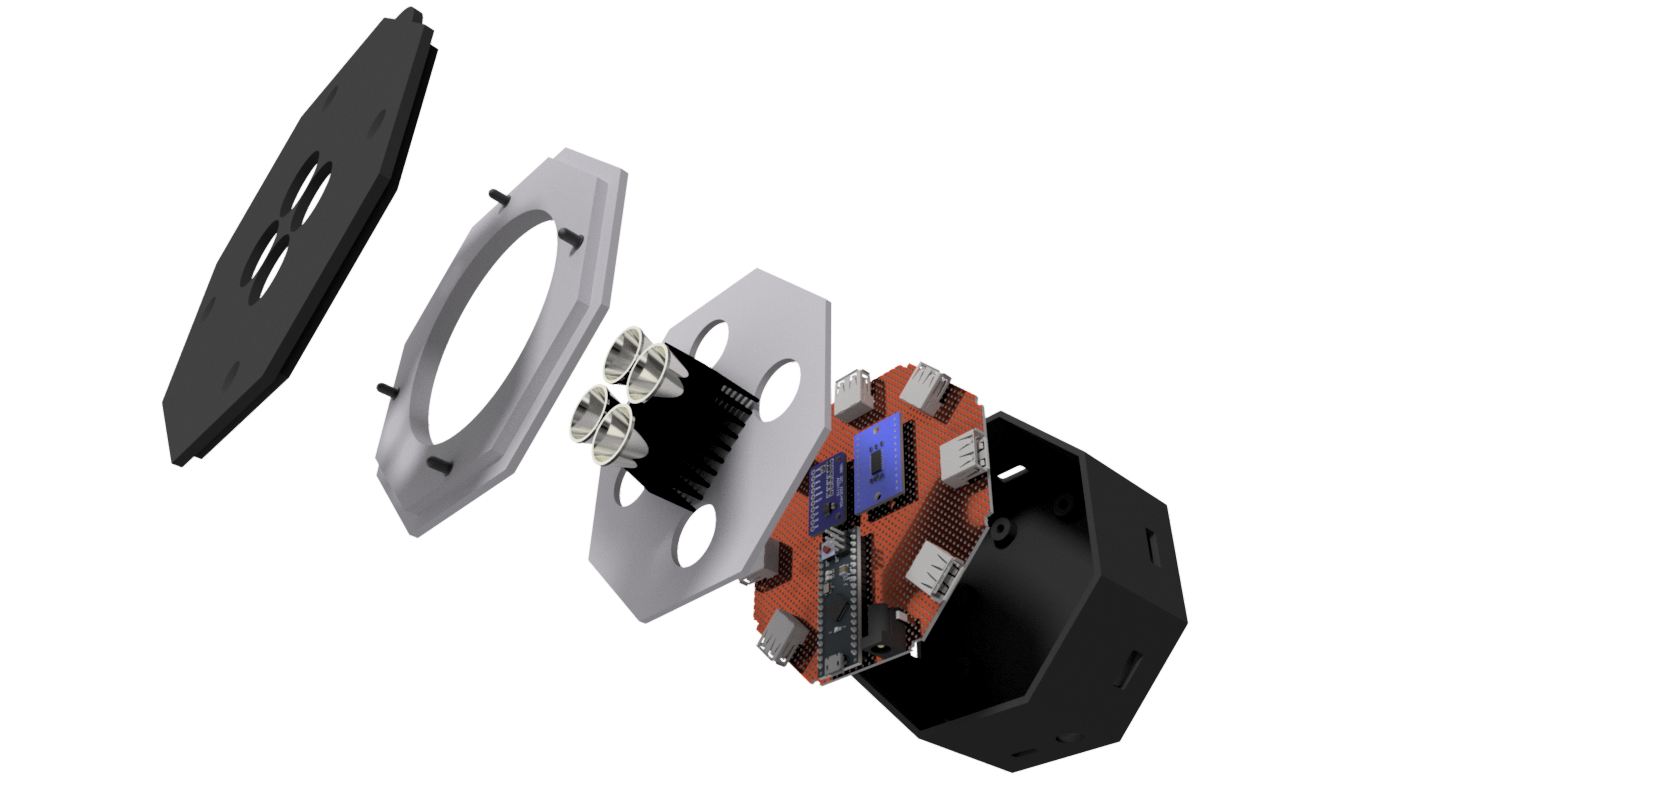
\includegraphics[scale=0.3]{../CAD_Bilder/Oktokommander/Oktokommander_raytraced.png}
	
	\vfill
	
\end{minipage}

\textcolor{rwth-lblue}{\noindent\rule{\textwidth}{4pt}}

\noindent
\begin{minipage}[c][0.32\textheight][t]{\textwidth}
	\begin{itemize}
		\item Robust gegenüber Umgebungslicht durch Verwendung von IR-Licht 
		\item Tag und Nacht einsatzbereit
		\item Portabel durch modulares Stecksystem
		\item Individuell auf die Geste des Nutzers anpassbar
		\item geringer Energieverbrauch durch Verwendung von rudimentären elektronischen Bauteilen
		\item plattformunabhängige Software
		\item Steuerung von Bluetooth-fähigen Endgeräten
	\end{itemize}
\end{minipage}

\clearpage


%%%%%%%%%%%%%%%%%%
%%% Third page %%%
%%%%%%%%%%%%%%%%%%

% Macht eine Doppelseite
\makebox[\linewidth][l]{
	\begin{minipage}{2.2\linewidth}

		\section{Funktionsweise} 
		
		\begin{tikzpicture}[fill=rwth-blue,ultra thick]
		
			\tikzstyle{myarrows}=[line width=1mm,draw=rwth-blue,-triangle 45,postaction={draw, line width=3mm, shorten >=4mm, -}]
		
			\clip (0,0) rectangle (18,-18);
			
			%\draw[help lines] (0,0) grid (18,-18);
			
			\node[above,align=center] (Text1) at (3,-3) { 1) \textbf{Steckmodule} ermöglichen \\ einen leichten Transport \\ und Aufbau };
			\node[below] (Bild1) at (3,-3) {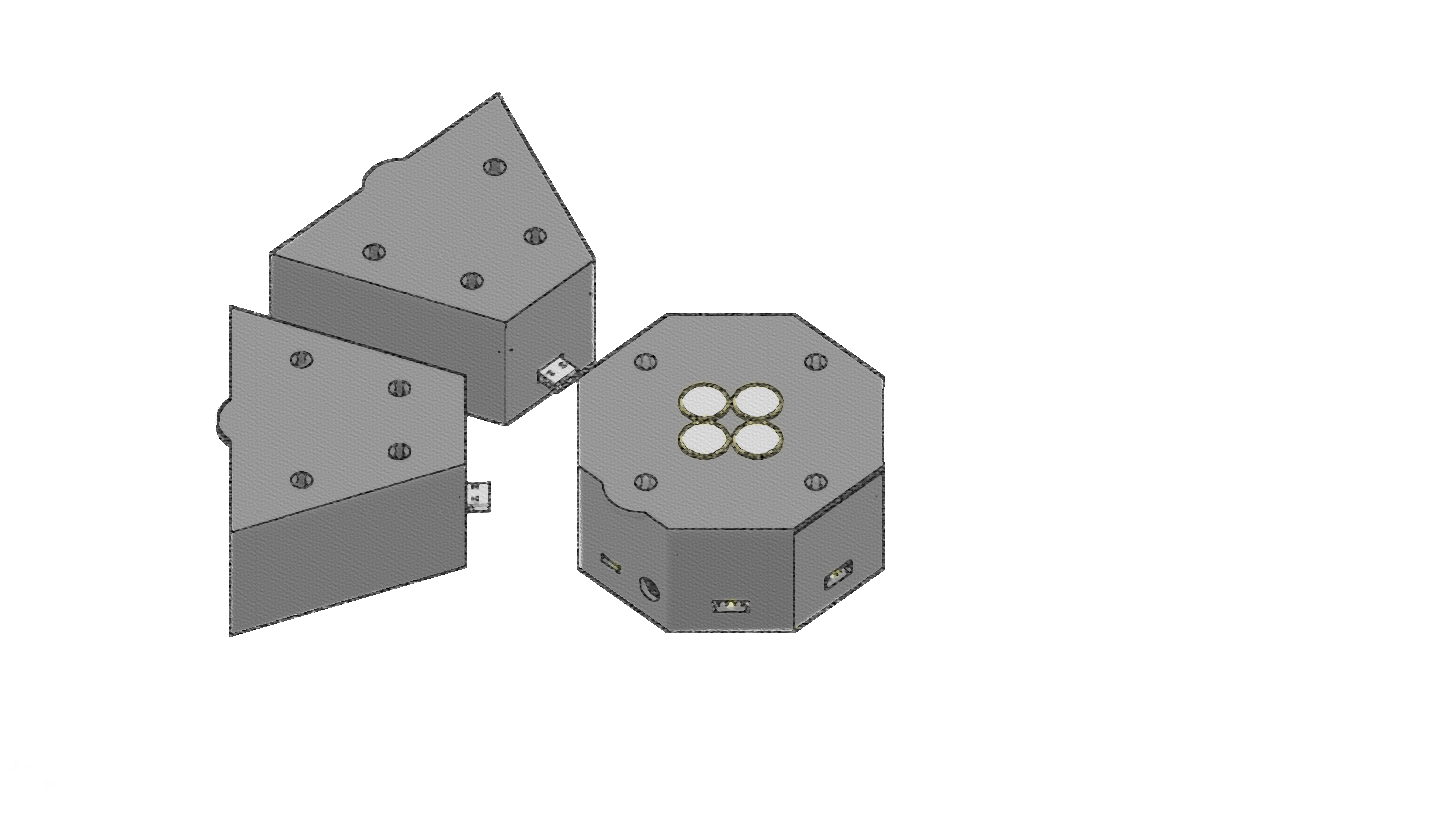
\includegraphics[scale=0.25]{../CAD_Bilder/Flyer_Bilder/IMG_1344.png}};
			
			\node[above,align=center] (Text2) at (13,-2.5) { 2) \textbf{Erkennen} einer \\ Handgeste durch \\ Detektion von \\ Lichtreflektionen };
			\node[below] (Bild2) at (13,-2.5) {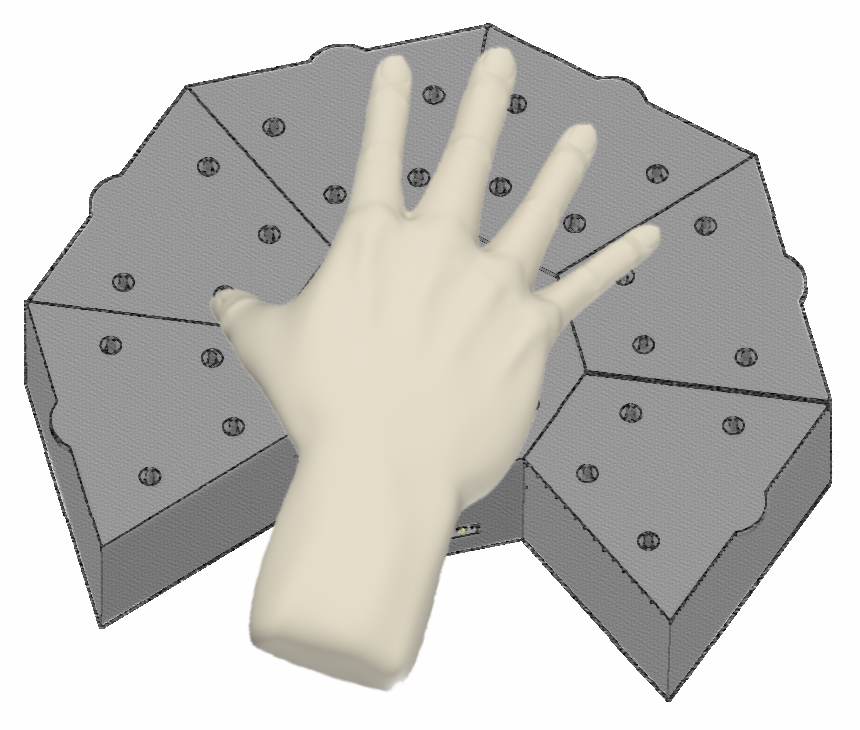
\includegraphics[scale=0.25]{../CAD_Bilder/Flyer_Bilder/IMG_1342.png}};
			
			\node[above,align=center] (Text3) at (13.5,-12) { 3) Interpretation der \\ Reflexionsmuster \\ mit Hilfe eines \\ \textbf{Machine Learning} \\ Algorithmus };
			\node[below] (Bild3) at (14,-12) {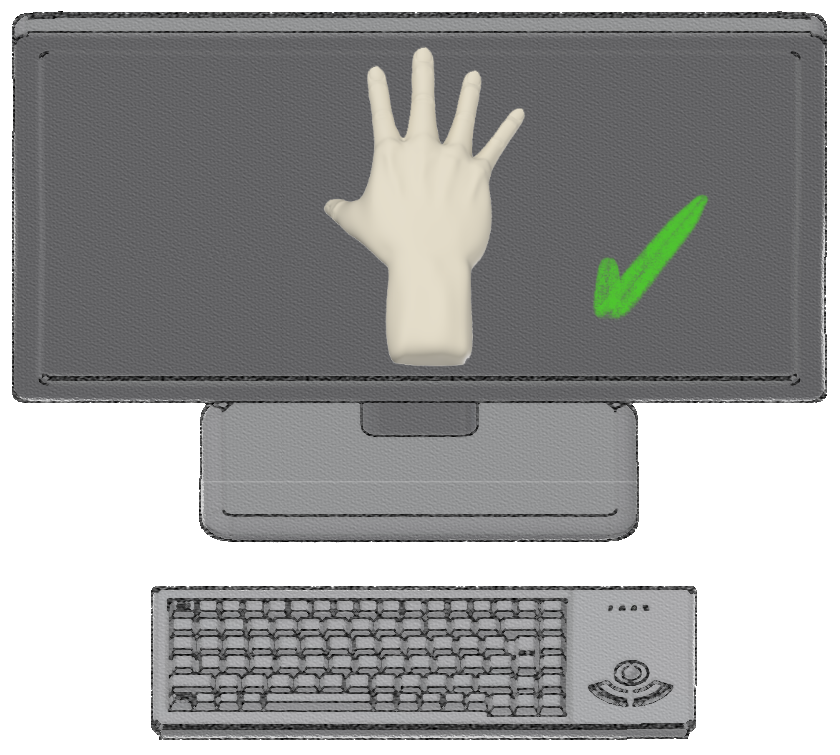
\includegraphics[scale=0.25]{../CAD_Bilder/Flyer_Bilder/IMG_1340.png}};
			
			\node[above,align=center] (Text4) at (4,-13) { 4) \textbf{Steuern} eines Endgeräts };
			\node[below] (Bild4) at (4,-13) {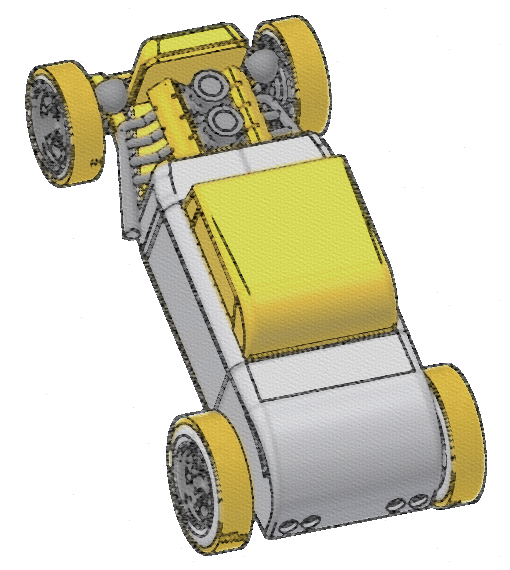
\includegraphics[scale=0.25]{../CAD_Bilder/Flyer_Bilder/IMG_1341.png}};
			
			\path[myarrows]
    			(Bild1) edge[bend left] node {} (Bild2);
    			
    		\path[myarrows]
    			(Bild2) edge[bend left] node {} (Bild3);
			
			\path[myarrows]
    			(Bild3) edge[bend left] node {} (Bild4);
			
		\end{tikzpicture}

	\end{minipage}
}

% Eine leere Seite (nötig wegen der Doppelseite)
\newpage
\thispagestyle{empty}
\quad 
\newpage


%%%%%%%%%%%%%%%%%%
%%% Fifth page %%%
%%%%%%%%%%%%%%%%%%

\noindent
\begin{minipage}[c][0.45\textheight][t]{\textwidth}
	
	\section{Unsere Zukunftsvision}
	
	\centering
	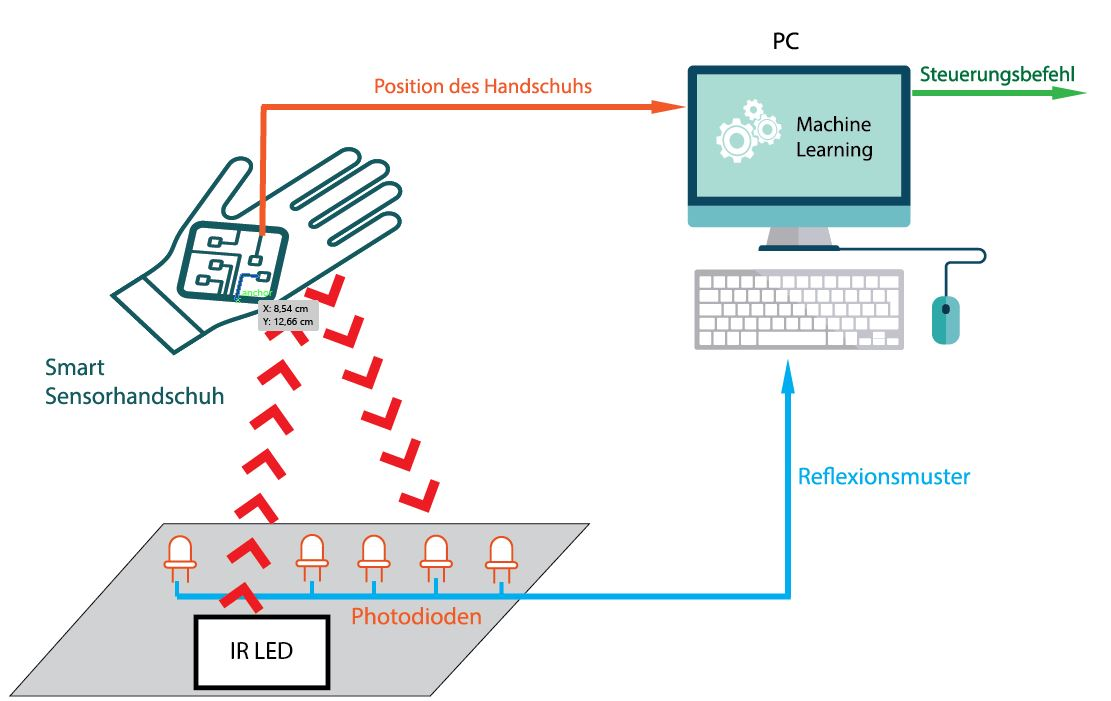
\includegraphics[scale=0.25]{../figures/AblaufGestikulaser3.jpg}
	%\textcolor{red}{Was kann noch verbessert werden und was ist unsere Vorstellung?}
	
\end{minipage}

\textcolor{rwth-lblue}{\noindent\rule{\textwidth}{4pt}}

\noindent
\begin{minipage}[c][0.45\textheight][t]{\textwidth}
	\begin{itemize}
		\item Verfeinerung der Gestenerkennung durch Verwendung eines Sensorhandschuhs in der Anlernphase
		\item Erkennung dynamischer Gesten
		\item Erzeugung eines individuellen Muster dank eines beliebig kombinierbaren Stecksystem
		\item Betrieb aus größerer Entfernung durch Verwendung von Laserlicht oder Lichtpulsen mit höherer Intensität
	\end{itemize}
\end{minipage}

\newpage


%%%%%%%%%%%%%%%%%%
%%% Sixth page %%%
%%%%%%%%%%%%%%%%%%

\noindent
\begin{minipage}[c][0.45\textheight][t]{\textwidth}
	\section{Das Team}
	\begin{description}
		\item[Projektleitung] Cailing Fu
		\item[Teammitglieder] Christoph Behr, \\ Nicole Grubert, Anna Pryadun, \\ Daniel Wolff
	\end{description}

	\section{Kontakt}
	\begin{description}
		\item[Kontaktperson] Cailing Fu 
		\item[Adresse] Fraunhofer-Institut für Lasertechnik, Steinbachstraße 15, 52074 Aachen
		\item[Telefon] +49 176 43404702
		\item[E-Mail] cailing.fu@rwth-aachen.de
	\end{description}
\end{minipage}

\textcolor{rwth-lblue}{\noindent\rule{\textwidth}{4pt}}

\noindent
\begin{minipage}[c][0.45\textheight][t]{\textwidth}
	\begin{center}
		\section{Sponsoren und Unterstützer}
		\vspace{0.7cm}
		
\includegraphics[height=1.25cm]{../Logos/Fraunhofer_ILT_klein.png} \\ \vspace{0.3cm}
		
\includegraphics[height=1.25cm]{../Logos/Wuerth.png} \\ \vspace{0.3cm}
		
\includegraphics[height=1.25cm]{../Logos/AC3D_Logo_Print-for-white.eps} \\ \vspace{0.3cm}
		
\includegraphics[height=1.25cm]{../Logos/BMBF.png} \\ \vspace{0.3cm}
		%
\includegraphics[height=0.5cm]{../Logos/Faulhaber.png} \\ \vspace{0.3cm}
		%
\includegraphics[height=1.5cm]{../Logos/micronit.jpg} \\ \vspace{0.3cm}
		
\includegraphics[height=1cm]{../Logos/electronica.png} \\ \vspace{0.3cm}
		
\includegraphics[height=0.8cm]{../Logos/VDE.png}
	\end{center}
\end{minipage}

\end{document}